%  Discussion.tex
% !TeX spellcheck = en_GB
% !TeX root = ReportMain.tex

\section{Discussion} \label{s:Discussion}
Comparison and discussion (Suggestions on improvement).
%BH
\subsection{Success Criteria}
What are the values the design must pass?

\subsection{No Foils}
\begin{figure}[!h]
  \centering
    \includegraphics[width = 0.8\textwidth]{../Simulations/DataSets/No_Foil_Fail.eps} 
\caption{The No Foils Model Fails PD Criteria}
\label{Figure:NoFoilsFail}
\end{figure}

\subsection{No Grading}

\subsection{Comparison of Axial and Radial Grading Solutions}
The design of both types of capacitive grading method were discussed in the previous sections. The difference in performance of the types in general is the radial grading will improve the intensity of the radial electric field and the axial grading will improve the intensity of the axial electric field. By improvement of intensity of electric field, this means the electric field according to the type of grading method is evenly distributed in a particular direction. Choosing the right design for different application is essential as this will reduce the chances of various types of electrical breakdown and hence the bushing design would be more durable.

There are two components of electric field cause different problems. The radial electric field is mainly responsible to the breakdown of insulating material, for example, electrical breakdown between foils. On the other hand, the axial electric field is mainly responsible to the surface discharges along the boundary of the insulation, for example, corona discharge to the surrounding.

\subsubsection{Radial Electric Field}
The maximum intensity of the radial electric field for the radial design is expected to be lower than the maximum of the axial design. This means the radial grading design would perform better to suppress the intensity of radial electric field. The radial electric field across the radial direction of both axial and radial grading designs are shown in figure \ref{figure:rfield}.

\begin{figure}[!h]
\centering
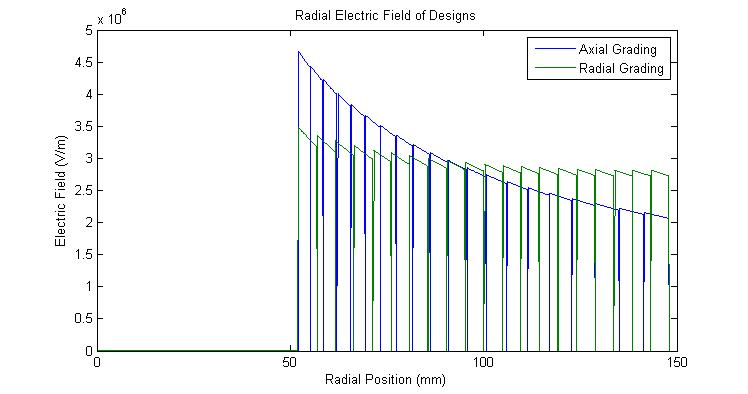
\includegraphics[width = \textwidth]{R-field.jpg}
\caption{Radial electric field across the mid-point of the two designs of bushing.}
\label{figure:rfield}
\end{figure}

The result clearly shows the peak value of electric field for the axial design ($\approx 4.5 \times 10^3 kVm^{-1}$) is greater than the peak value of electric field for the radial design ($\approx 3.5 \times 10^3 kVm^{-1}$).

\subsubsection{Axial Electric Field}

\subsubsection{Surface Flashover}

\subsection{Choice of Design Method}

\section{Conclusions}
Conclusions.